\documentclass[12pt]{ociamthesis}  % default square logo 
%\documentclass[12pt,beltcrest]{ociamthesis} % use old belt crest logo
%\documentclass[12pt,shieldcrest]{ociamthesis} % use older shield crest logo

%load any additional packages
\usepackage{amssymb}
\usepackage{listings}

%input macros (i.e. write your own macros file called mymacros.tex 
%and uncomment the next line)
%\include{mymacros}

\title{Modul Praktikum \\[1ex]     %your thesis title,
        Kecerdasan Buatan}   %note \\[1ex] is a line break in the title

\author{Rolly Maulana Awangga}             %your name
\college{0410118609\\[5ex]
Applied Bachelor of Informatics Engineering}  %your college

%\renewcommand{\submittedtext}{change the default text here if needed}
\degree{Politeknik Pos Indonesia}     %the degree
\degreedate{Bandung 2019}         %the degree date

%end the preamble and start the document
\begin{document}

%this baselineskip gives sufficient line spacing for an examiner to easily
%markup the thesis with comments
\baselineskip=18pt plus1pt

%set the number of sectioning levels that get number and appear in the contents
\setcounter{secnumdepth}{3}
\setcounter{tocdepth}{3}


\maketitle                  % create a title page from the preamble info
\include{section/dedication}        % include a dedication.tex file
\include{section/acknowlegements}   % include an acknowledgements.tex file
\include{section/abstract}          % include the abstract

\begin{romanpages}          % start roman page numbering
\tableofcontents            % generate and include a table of contents
\listoffigures              % generate and include a list of figures
\end{romanpages}            % end roman page numbering

%now include the files of latex for each of the chapters etc
\include{section/chapter1}
\include{section/chapter2}
\chapter{Methods}
\extrafloats{100}
\maxdeadcycles=200

\section{The data}
PLease tell where is the data come from, a little brief of company can be put here.

\section{Method 1}
Definition, steps, algoritm or equation of method 1 and how to apply into your data
\section{Method 2}
Definition, steps, algoritm or equation of method 2 and how to apply into your data

\section{Andri Fajar Sunandhar/1164065}a
\subsection{Teori}
\begin{enumerate}
\item Apa itu Random Forest Serta Gambar Ilustrasinya \par
Random Forest adalah suatu algoritma yang digunakan pada klasifikasi data dalam jumlah yang besar. Klasifikasi random forest dilakukan melalui penggabungan pohon  dengan melakukan training pada sampel data yang dimiliki. Penggunaan tree yang semakin banyak akan mempengaruhi akurasi yang akan didapatkan menjadi lebih baik. Penentuan klasifikasi dengan random forest diambil berdasarkan hasil voting dari pohon yang terbentuk. Pemenang dari pohon yang terbentuk ditentukan dengan vote terbanyak. Pembangunan pohon  pada random forest sampai dengan mencapai ukuran maksimum dari pohon data. Akan tetapi, pembangunan pohon Random Forest tidak dilakukan pemangkasan  yang merupakan sebuah metode untuk mengurangi kompleksitas ruang. Contoh Ilustrasi sederhana Gambar Random Forest. 
		\begin{figure}[ht]
		\centerline{\includegraphics[width=1\textwidth]{figures/AFS/AFS1.png}}
		\caption{Random Forest.}
		\label{AFS1}
		\end{figure}

\item Cara Membaca Dataset
	

		\begin{enumerate}
			\item Buka Anaconda Navigator.
			\item Jalankan Spyder
			\item Import libraries yang dibutuhkan
			\item Masukan kode berikut untuk membaca file Data.csv.
				\begin{figure}[ht]
				\centering
				\includegraphics[scale=0.8]{figures/AFS/2.png}
				\caption{Kode membaca file.csv}
				\label{contoh}
				\end{figure}
			\item Jalankan kode tersebut, maka di windiws console akan muncul pesan :
				\begin{figure}[ht]
				\centering
				\includegraphics[scale=0.9]{figures/AFS/3.png}
				\caption{ Window Console}
				\label{contoh}
				\end{figure}
			\item Klik variable explorer, maka akan terlihat dataset yang baru ter-import.
				\begin{figure}[ht]
				\centering
				\includegraphics[scale=0.6]{figures/AFS/4.png}
				\caption{Variable Explorer}
				\label{contoh}
				\end{figure}
			\item Kemudian double klik pada dataset cell, maka akan muncul pop-up windows seperti berikut: 
				\begin{figure}[ht]
				\centering
				\includegraphics[scale=0.7]{figures/AFS/5.png}
				\caption{ Dataset Cell}
				\label{contoh}
				\end{figure}
			\item Seperti yang terlihat pada gambar tersebut dataset ini memiliki Kolom Country, Age, dan Salary sebagai 		   				independent variable-nya dan kolom Purchased sebagai dependent variable-nya.			
		\end{enumerate}
	

\item Cross Validation \par
Cross validation adalah metode statistik yang digunakan untuk memperkirakan keterampilan model pembelajaran mesin. Ini biasanya digunakan dalam pembelajaran mesin yang diterapkan untuk membandingkan dan memilih model untuk masalah pemodelan prediktif yang diberikan karena mudah dipahami, mudah diimplementasikan, dan menghasilkan estimasi keterampilan yang umumnya memiliki bias lebih rendah daripada metode lainnya.

\item Arti Score 44\% Pada Random Forest, 27\% Pada Decision Tree dan 29\% Dari SVM \par
	\begin{enumerate}
	\item Arti Score 44\% \par Pada Random Forest, Score tersebut merupakan hasil dari akurasi.
	\item Arti Score 27\% \par Pada decission tree adalah presentasi hasil dari perhitungan dataset.
	\item Arti Score 29\% Pada SVM \par merupakan hasil pendekatan jaringan saraf. Jaringan saraf sendiri merupakan komponen jaringan utama dari sistem saraf. Sistem tersebut mengatur dan mengontrol fungsi tubuh dan aktivitas dan terdiri dari dua bagian:  (SSP) yang terdiri dari otak dan sumsum tulang belakang, dan percabangan saraf perifer dari sistem saraf tepi (SST) yang terdapat dalam pengolahan dataset terkait. 
	\end{enumerate}

\begin {enumerate}
\item Confusion Matrix Dan Ilustrasinya
\end{enumerate}

\begin{enumerate}
\item Perhitungan confusion matrix adalah sebagai berikut, akan saya beri contoh sederhana yaitu pengambilan keputusan untuk mendapatkan bantuan beasiswa. Saya menggunakan dua atribut, yaitu rekening listrik dan gaji. Ini adalah pohon keputusannya:
 
\begin{figure}[ht]
\centering
\includegraphics[scale=0.5]{figures/AFS/7.jpg}
\caption{Pohon Keputusan}
\label{contoh}
\end{figure}

\end{enumerate}


Kemudian data testingnya adalah

\begin{figure}[ht]
\centering
\includegraphics[scale=0.5]{figures/AFS/8.jpg}
\caption{Data Testing}
\label{contoh}
\end{figure}

Yang pertama kita lakukan yaitu mencari 4 nilai yaitu a,b,c, dan d:

 a= 5

 b= 1

 c= 1

 d= 3

Kemudian kita dapat mencari nilai Recall, Precision, accuracy dan Error Rate

 Recall =3/(1+3) = 0,75

 Precision = 3/(1+3) = 0,75

 Accuracy =(5+3)/(5+1+1+3) = 0,8

 Error Rate =(1+1)/(5+1+1+3) = 0,2

\item Jelaskan Voting Pada Random Forest Beserta Ilustrasinya 
\par Voting merupakan metode yang paling umum digunakan dalam random forest. Ketika classifier membuat keputusan, Anda dapat memanfaatkan yang terbaik keputusan umum dan rata-rata yang didefinisikan ke dalam bentuk "voting". Setelah pohon terbentuk,maka akan dilakukan voting pada setiap kelas dari data sampel. Kemudian, mengkombinasikan vote dari setiap kelas kemudian diambil vote yang paling banyak. Dengan menggunakan random forest pada klasifikasi data maka, akan menghasilkan vote yang paling baik. \ref{AFS6}
		\begin{figure}[ht]
		\centerline{\includegraphics[width=1\textwidth]{figures/AFS/6.png}}
		\caption{Voting.}
		\label{AFS6}
		\end{figure}



\subsection{Praktek Program}
\begin{enumerate}
\item Aplikasi Sederhana Menggunakan Pandas
	\begin{figure}[ht]
	\centering
	\includegraphics[scale=0.5]{figures/AFS/praktek1.jpg}
	\caption{Aplikasi Pandas}
	\label{contoh}
	\end{figure}

\end{enumerate}
	\par Penjelasan kodingan :
		\begin{enumerate}
		\item Memanggil library.
		\item Membuat variable dengan data frame.
		\item Menampilkan hasil
		\end{enumerate}
	\par Sehingga menghasilkan :
	\begin{figure}[ht]
	\centering
	\includegraphics[scale=0.5]{figures/AFS/praktek2.jpg}
	\caption{Hasil Pandas}
	\label{contoh}
	\end{figure}
\item Aplikasi Sederhana Menggunakan Numpy
	\begin{figure}[ht]
	\centering
	\includegraphics[scale=0.5]{figures/AFS/praktek3.png}
	\caption{Aplikasi Numpy}
	\label{contoh}
	\end{figure}
	\par Penjelasan kodingan :
		\begin{enumerate}
		\item Memanggil library numpy
		\item Membuat variable dengan value eye dengan size10
		\item Menampilkan hasil value
		\end{enumerate}
	\par Sehingga menghasilkan :
	\begin{figure}[ht]
	\centering
	\includegraphics[scale=0.5]{figures/AFS/praktek4.png}
	\caption{Hasil Numpy}
	\label{contoh}
	\end{figure}
\item Aplikasi Sederhana Menggunakan Matplotlib
	\begin{figure}[ht]
	\centering
	\includegraphics[scale=0.5]{figures/AFS/praktek5.png}
	\caption{Aplikasi Matplotlib}
	\label{contoh}
	\end{figure}
	\par Penjelasan kodingan :
		\begin{enumerate}
		\item Memanggil library matplotlib.pyplot
		\item Membuat variable yang berisi 10,20,30,40,50,60,70
		\item Membuat garis koordinat
		\item Menampilkan hasil plt
		\end{enumerate}
	\par Sehingga menghasilkan :
	\begin{figure}[ht]
	\centering
	\includegraphics[scale=0.5]{figures/AFS/praktek6.png}
	\caption{Hasil Matplotlib}
	\label{contoh}
	\end{figure}
\par
\par
\item Program Klasifikasi Random Forest :
\begin{itemize}
\item Code Random Forest 1 :
\par
\begin{figure}[ht]
\centering
\includegraphics[scale=0.7]{figures/AFS/4a.jpg}
\caption{Gambar1}
\label{contoh}
\end{figure}
\par
\end{itemize}

\begin{itemize}
\item Penjelasan : Membaca dataset. Codingan di atas menghasilkan variabel baru yaitu imgatt. Terdapat 3 kolom dan 3677856 baris data.
\par 
\par
\end{itemize}
\item Code Random Forest 2 :
\par
\begin{figure}[ht]
\centering
\includegraphics[scale=0.7]{figures/AFS/4b.jpg}
\caption{Gambar2}
\label{contoh}
\end{figure}
\par
\begin{itemize}
\item Penjelasan : Codingan di atas berfungsi untuk melihat sebagian data awal dari dataset. Hasilnya terdapat pada gambar di atas setelah di eksekusi.
\par
\par
\end{itemize}
\item Code Random Forest 3 :
\par
\begin{figure}[ht]
\centering
\includegraphics[scale=0.7]{figures/AFS/4c.jpg}
\caption{Gambar3}
\label{contoh}
\end{figure}
\par
\begin{itemize}
\item Penjelasan : Codingan di atas merupakan tampilan untuk menampilkan hasil dari dataset yang telah di run atau di eksekusi. Dimana pada gambar di atas 3677856 merupakan baris dan 3 adalah kolom.
\par
\par
\end{itemize}
\item Code Random Forest 4 :
\par
\begin{figure}[ht]
\centering
\includegraphics[scale=0.7]{figures/AFS/4d.jpg}
\caption{Gambar 4}
\label{contoh}
\end{figure}
\par
\begin{itemize}
\item Penjelasan : Pada gambar di atas menmapilkan hasil dari variabel imgatt2. Dimana index nya 'imgid', kolom berisi 'attid' dan values atau nilainya berisi 'present'.
\par
\par
\end{itemize}
\item Code Random Forest 5 :
\par
\begin{figure}[ht]
\centering
\includegraphics[scale=0.7]{figures/AFS/4e.jpg}
\caption{Gambar 5}
\label{contoh}
\end{figure}
\par
\begin{itemize}
\item Penjelasan : Pada gambar di atas menmapilkan hasil dari variabel imgatt2.head. Dimana dataset nya ada 5 baris dan 312 kolom.
\par
\par
\end{itemize}
\item Code Random Forest 6 :
\par
\begin{figure}[ht]
\centering
\includegraphics[scale=0.7]{figures/AFS/4f.jpg}
\caption{Gambar 6}
\label{contoh}
\end{figure}
\par
\begin{itemize}
\item Penjelasan : Pada gambar di atas menampilkan jumlah dari baris dan kolom dari variabel imgatt2. Dimana 11788 adalah baris dan 312 adalah kolom.
\par
\par
\end{itemize}
\item Code Random Forest 7 :
\par
\begin{figure}[ht]
\centering
\includegraphics[scale=0.7]{figures/AFS/4g.jpeg}
\caption{Gambar 7}
\label{contoh}
\end{figure}
\par
\begin{itemize}
\item Penjelasan : Pada gambar di atas menunjukkan load dari  jawabannya yang berisi " apakah burung tersebut ( subjek pada dataset ) termasuk dalam spesies yang mana ?. Kolom yang digunakan adalah imgid dan label, kemudian melakukan pivot yang mana imgid menjadi index yang artinya unik sehubungan dengan dataset yang telah dieksekusi.
\par
\par
\end{itemize}
\item Code Random Forest 8 :
\par
\begin{figure}[ht]
\centering
\includegraphics[scale=0.2]{figures/AFS/4h.jpg}
\caption{Gambar 8}
\label{contoh}
\end{figure}
\par
\begin{itemize}
\item Penjelasan : Pada gambar di atas menunjukkan hasil dari variabel imglabels. Dimana menampilkan dataset dari imgid dan label. Dan dapat dilihat hasilnya dari gambar di atas.
\par
\par
\end{itemize}
\item Code Random Forest 9 :
\par
\begin{figure}[ht]
\centering
\includegraphics[scale=0.7]{figures/AFS/4i.jpg}
\caption{Gambar 9}
\label{contoh}
\end{figure}
\par
\begin{itemize}
\item Penjelasan : Pada gambar di atas menunjukkan jumlah baris dan kolom dari variabel imglabels. Dimana hasil dari kodingan tersebut dapat dilihat setelah di run. 
\par
\par
\end{itemize}
\item Code Random Forest 10 :
\par
\begin{figure}[ht]
\centering
\includegraphics[scale=0.7]{figures/AFS/4j.jpg}
\caption{Gambar 10}
\label{contoh}
\end{figure}
\par
\begin{itemize}
\item Penjelasan : Pada gambar diatas dikarenakan isinya sama, maka bisa melakukan join antara dua data yang diesekusi ( yaitu ada imgatt2 dan imglabels ), sehingga pada hasilnya akan didapatkan data ciri dan data jawaban atau labelnya sehingga bisa dikategorikan/dikelompokkan sebagai supervised learning. Jadi perintah untuk menggabungkan kedua data, kemudian dilakukan pemisahan antara data set untuk training dan test pada dataset yang dieksekusi.
\par
\par
\end{itemize}
\item Code Random Forest 11 :
\par
\begin{figure}[ht]
\centering
\includegraphics[scale=0.7]{figures/AFS/4k.jpg}
\caption{Gambar 11}
\label{contoh}
\end{figure}
\par
\begin{itemize}
\item Penjelasan :Pada gambar di atas menghasilkan pemisahan dan pemilihan tabel ( memisahkan dan memilih tabel ). 
\par
\par
\end{itemize}
\item Code Random Forest 12 :
\par
\begin{figure}[ht]
\centering
\includegraphics[scale=0.7]{figures/AFS/4l.jpg}
\caption{Gambar 12}
\label{contoh}
\end{figure}
\par
\begin{itemize}
\item Penjelasan : Pada gambar di atas menunjukkan hasil dari variabel dtatthead. Dimana data nya dapat dilihat pada gambar diatas. Dan dataset nya terdiri dari 5 baris dan 312 kolom.
\par
\par
\end{itemize}
\item Code Random Forest 13 :
\par
\begin{figure}[ht]
\centering
\includegraphics[scale=0.7]{figures/AFS/4m.jpg}
\caption{Gambar 13}
\label{contoh}
\end{figure}
\par
\begin{itemize}
\item Penjelasan : Pada gambar di atas menunjukkan hasil dari variabel dflabel.head. Dimana berisikan data dari imgid dan label. Dan hasilnya dapat dilihat pada gambar di atas.
\par
\par
\end{itemize}
\item Code Random Forest 14 :
\par
\begin{figure}[ht]
\centering
\includegraphics[scale=0.7]{figures/AFS/4n.jpg}
\caption{Gambar 14}
\label{contoh}
\end{figure}
\par
\begin{itemize}
\item Penjelasan : Pada gambar di atas merupakan pembagian dari data training dan dataset
\par
\par
\end{itemize}
\item Code Random Forest 15 :
\par
\begin{figure}[ht] 
\centering
\includegraphics[scale=0.7]{figures/AFS/4o.jpg}
\caption{Gambar 15}
\label{contoh}
\end{figure}
\par
\begin{itemize} 
\item Penjelasan : Pada gambar di atas merupakan pemanggilan kelas RandomForestClassifier. max features yang diartikan berapa banyak kolom pada setiap tree.
\par
\par
\end{itemize}
\item Code Random Forest 16 :
\par
\begin{figure}[ht]
\centering
\includegraphics[scale=0.7]{figures/AFS/4p.jpg}
\caption{Gambar 16}
\label{contoh}
\end{figure}
\par
\begin{itemize}
\item Penjelasan : Pada gambar di atas merupaka perintah untuk melakukan fit untuk membangun random forest yang sudah ditentukan dengan maksimum fitur sebanyak 50.
\par
\par
\end{itemize}
\item Code Random Forest 17 :
\par
\begin{figure}[ht]
\centering
\includegraphics[scale=0.7]{figures/AFS/4q.jpg}
\caption{Gambar 17}
\label{contoh}
\end{figure}
\par
\begin{itemize}
\item Penjelasan : Pada gambar di atas menunjukkan hasil dari cetakan variabel dftrainatt.head.
\par
\par
\end{itemize}
\item Code Random Forest 18 :
\par
\begin{figure}[ht]
\centering
\includegraphics[scale=0.7]{figures/AFS/4r.jpg}
\caption{Gambar 18}
\label{contoh}
\end{figure}
\par
\begin{itemize}
\item Penjelasan : Pada gambar di atas merupakan hasil dari variabel dftestatt da dftsetlabel. Dimana hasilnya dapat dilihat dari pada gambar di atas
\par
\par
\end{itemize}

\item Program Klasifikasi Confusion Matrix
	\begin{itemize}
		\item Setelah melakukan random forest kemudian dipetakan ke dalam confusion matrix.
			\begin{figure}[ht]
			\centering
			\includegraphics[scale=0.5]{figures/AFS/abc1.jpg}
			\caption{Memetakan ke confusion matrix}
			\label{contoh}
			\end{figure}
		\item Lalu melihat hasilnya.
			\begin{figure}[ht]
			\centering
			\includegraphics[scale=0.5]{figures/AFS/abc2.jpg}
			\caption{Melihat hasil}
			\label{contoh}
			\end{figure}
		\item Kemudian dilakukan perintah plot.
			\begin{figure}[ht]
			\centering
			\includegraphics[scale=0.5]{figures/AFS/abc3.jpg}
			\caption{Melakukan Plot}
			\label{contoh}
			\end{figure}
		\item Selanjutnya nama data akan di set agar plot sumbunya sesuai.
			\begin{figure}[ht]
			\centering
			\includegraphics[scale=0.5]{figures/AFS/abc4.jpg}
			\caption{Plotting nama data}
			\label{contoh}
			\end{figure}
		\item Setelah label berubah, maka dilakukan perintah plot.
		\begin{figure}[ht]
			\centering
			\includegraphics[scale=0.5]{figures/AFS/abc5.jpg}
			\caption{Melakukan perintah plot}
			\label{contoh}
			\end{figure}
	\end{itemize}
\par
\par
\item Program Klasifikasi SVM dan Decision Tree Beserta Penjelasan Keluarannya :
\begin{itemize}
\item Code SVM :
\par
\begin{figure}[ht]
\centering
\includegraphics[scale=0.7]{figures/AFS/t2.jpg}
\caption{SVM}
\label{contoh}
\end{figure}
\par
\end{itemize}

\begin{itemize}
\item Penjelasan : Pada gambar di atas cara untuk mencoba klasikasi dengan SVM dengan dataset yang sama.
\par 
\par
\end{itemize}
\item Code Decision Tree :
\par
\begin{figure}[ht]
\centering
\includegraphics[scale=0.7]{figures/AFS/t1.jpg}
\caption{Decission Tree}
\label{contoh}
\end{figure}
\par
\begin{itemize}
\item Penjelasan : Pada gambar di atas merupakan cara untuk mencoba klasikasi dengan decission tree dengan dataset yang sama.
\par
\par

\end{itemize}


\item Program Cross Validation
	\begin{itemize}
		\item Melakukan pengecekan cross validation untuk random forest.
			\begin{figure}[ht]
			\centering
			\includegraphics[scale=0.5]{figures/AFS/fajar1.jpg}
			\caption{Pengecekan cross validation random forest}
			\label{contoh}
			\end{figure}
		\item Melakukan pengecekan cross validation untuk decission tree.
			\begin{figure}[ht]
			\centering
			\includegraphics[scale=0.5]{figures/AFS/fajar2.jpg}
			\caption{Pengecekan cross validation decision tree}
			\label{contoh}
			\end{figure}
		\item Melakukan pengecekan cross validation untuk SVM.
	\end{itemize}

\item Program Pengamatan Komponen Informasi
	\begin{itemize}
		\item Melakukan pengamatan komponen informasi untuk menetahui berapa banyak tree yang dibuat, atribut yang dipakai, dan informasi lainnya.
			\begin{figure}[ht]
			\centering
			\includegraphics[scale=0.5]{figures/AFS/sunandhar1.jpg}
			\caption{Pengamatan Komponen}
			\label{contoh}
			\end{figure}
		\item Melakukan plot informasi agar bisa dibaca.
			\begin{figure}[ht]
			\centering
			\includegraphics[scale=0.5]{figures/AFS/sunandhar2.jpg}
			\caption{Plot informasi}
			\label{contoh}
			\end{figure}
	\end{itemize}
\end{enumerate}

\par
\par
\subsection{Penanganan Eror}
Penyelesaian Tugas Harian  ( Penanganan Error )
\begin{enumerate}
\item Menyelesaikan dan Membahas Penanganan Error :
\begin{itemize}
\item Skrinsut Error

\begin{figure}[ht]
\centering
\includegraphics[scale=0.7]{figures/AFS/Error.jpg}
\caption{Error}
\label{contoh}
\end{figure}
\end{itemize}

\begin{itemize}
\item Kode Error: file b'data/CUB 200 2011/attributes/image attributes labels.txt'
\par 
\item Solusi Pemecahan Error : Hapus Direktori data pada kode pastikan satu folder.
\par 
\par
\end{itemize}
\end{enumerate}

\chapter{Experiment and Result}
brief of experiment and result.
\section{Experiment}
Please tell how the experiment conducted from method.

\section{Result}
Please provide the result of experiment

\section{Andri Fajar Sunandhar/1164065}

\subsection{Teori}
\begin{enumerate}
\item Klasifikasi teks
	\par Klasifikasi Teks adalah salah satu tugas penting dan tipikal dalam supervised machine learning (ML). Teks dapat menjadi sumber informasi yang sangat kaya, tetapi mengekstraksi wawasan darinya bisa sulit dan memakan waktu karena sifatnya yang tidak terstruktur.
	\begin{figure}[ht]
		\centering
		\includegraphics[scale=0.5]{figures/AFS/k1.png}
		\caption{Klasifikasi teks}
		\label{contoh}
	\end{figure}
	
\item Mengapa Klasifikasi Bunga tidak dapat menggunakan machine learning
	\par Dikarenakan tidak semua bunga memliki ciri - ciri yang sama. Atau dalam kata lain terdapat data noise dalam klasifikasi bunga sehingga tidak bisa menggunakan machine learning.
	\begin{figure}[ht]
		\centering
		\includegraphics[scale=0.5]{figures/AFS/k2.png}
		\caption{Klasifikasi bunga}
		\label{contoh}
	\end{figure}

\item Teknik pembelajaran mesin pada teks YouTube
	\par Kita ambil sebuah kasus yang semua orang telah ketahui dan juga pahami. Kasus tersebut yaitu perekomendasian video dari pencarian menggunakan "text / kata" di  Youtube. Pada saat menggunakan Youtube terdapat Mchine Learning yang bekerja dan memproses perintah ataupun aktivitas tersebut, dimana akan memfilter secara otomatis video yang disesuaikan dengan "keyword" yang kita masukkan sehingga memberikan keluaran video dengan keyword yang benar. Adapula pada saat kita sedang menonton video di YouTube, pada bagian sebelah kanan ( tampilan Youtube ) terdapat 'Up Next' yang menampilkan beberapa video serupa yang sedang ditonton. Dan ketika mengklik salah satu video dari baris tersebut, maka YouTube akan mengingatnya dan menggunakan kata yang tertera sebagai referensi kembali sehingga akan memberikn kemudahan pada pencarian yang lannya, Dan disitulah mesin belajar sendiri dan menyimpan data secara berkala sehingga berkembang. 

	\begin{figure}[ht]
		\centering
		\includegraphics[scale=0.5]{figures/AFS/k3.jpeg}
		\caption{Teknik YouTube}
		\label{contoh}
	\end{figure}

\item Vectorisasi Data
	\begin{itemize}
		\item Pembagian dan pemecahan data, dan kemudian dilakukan perhitungan datanya. Vektorisasi juga dapat dimaksudkan dengan setiap data yang mungkin dipetakan ke integer tertentu. Yang mana data tersebut dalam bentuk data vektor diperoleh dalam bentuk koordinat titik yang menampilkan, menempatkan dan menyimpan data spasial dengan menggunakan titik, garis atau area (poligon). 
	\end{itemize}
	
\item Bag of word
	\par Bag-of-words ialah sebuah gambaran sederhana digunakan dalam pengolahan bahasa alami dan pencarian informasi. Dikenal sebagai model ruang vektor. Pada model ini, tiap kalimat dalam dokumen digambarkan sebagai token, mengabaikan tata bahasa dan bahkan urutan kata namun menghitung frekuensi kejadian atau kemunculan kata dari dokumen.
	\begin{figure}[ht]
		\centering
		\includegraphics[scale=0.5]{figures/AFS/k4.png}
		\caption{Bag of Word}
		\label{contoh}
	\end{figure}
	
\item TF-IDF
	\par TF-IDF atau TFIDF, adalah kependekan dari istilah frekuensi dokumen terbalik, dimana merupakan statistik numerik yang dimaksudkan untuk mencerminkan betapa pentingnya sebuah kata untuk sebuah dokumen dalam kumpulan atau kumpulan. Nilai tf-idf meningkat secara proporsional dengan berapa kali sebuah kata muncul dalam dokumen dan diimbangi dengan jumlah dokumen dalam korpus yang mengandung kata, yang membantu menyesuaikan fakta bahwa beberapa kata muncul lebih sering secara umum.
	\begin{figure}[ht]
		\centering
		\includegraphics[scale=0.5]{figures/AFS/k5.jpeg}
		\caption{TF IDF}
		\label{contoh}
	\end{figure}
\end{enumerate}


\subsection{Praktek Program}
\begin{enumerate}
\item Aplikasi sederhana menggunakan pandas
	\par Berikut adalah contoh aplikasi sederhana yang dibuat menggunakan pandas :
	
		\begin{figure}[ht]
		\centering
		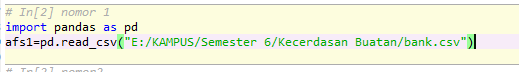
\includegraphics[scale=0.5]{figures/AFS/a1.png}
		\caption{Pandas}
		\label{contoh}
		\end{figure}
		
	\begin{enumerate}
	\item 1 = memanggil library pandas sebagai pd
	\item 2 = membuat varible afs1 untuk membaca file .csv (bank.csv)
	\end{enumerate}
	
	\par Hasil dari pandas menampilkan data dari bank.csv :
	
		\begin{figure}[ht]
		\centering
		\includegraphics[scale=0.5]{figures/AFS/a2.png}
		\caption{Hasil Pandas}
		\label{contoh}
		\end{figure}	
	
\item Memecah dataframe menjadi 2 dataframe
	\par Memecah dataframe :
	
		\begin{figure}[ht]
		\centering
		\includegraphics[scale=0.5]{figures/AFS/a3.png}
		\caption{Memecah dataframe}
		\label{contoh}
		\end{figure}
	
	\begin{enumerate}
	\item 1 = Melakukan split data training sebanyak 450
	\item 2 = dan sisanya sebagai data testing
	\end{enumerate}
	
	\par Berikut hasil memecah dataframe menjadi 2 :
	
		\begin{figure}[ht]
		\centering
		\includegraphics[scale=0.5]{figures/AFS/a4.png}
		\caption{Hasil memecah dataframe}
		\label{contoh}
		\end{figure}
		
\item Vektorisasi dan klasifikasi Decission Tree dari data Youtube03-LMFAO.csv
	
	\par Berikut adalah vektorisasi dan klasifikasi dari data Youtube03-LMFAO.csv
		\begin{figure}[ht]
		\centering
		\includegraphics[scale=0.5]{figures/AFS/a5.png}
		\caption{Vektorisasi dan klasifikasi}
		\label{contoh}
		\end{figure}
	\begin{enumerate}
	\item 1 = Melakukan import pandas dan membaca file Youtube03-LMFAO.csv
	\item 2 = Mengelompokan data spam bukan spam
	\item 3 = Memanggil library vektorisasi dan menghitung kata yang muncul per kalimat
	\item 4 = Memilih kolom CONTENT untuk melakukan vektorisasi
	\item 5 = Melihat isi vektorisasi
	\item 6 = Melihat isi data pada kolom CONTENT namun pada bagian kolom ke 349
	\item 7 = Melihat daftar kata yang di vektorisasi
	\item 8 = Akan melakukan pengocokan pada data nya supaya hasilnya sempurna ketika melakukan klasifikasi
	\end{enumerate}
	
	\par Berikut adalah Decission Tree Youtube03-LMFAO.csv
		\begin{figure}[ht]
		\centering
		\includegraphics[scale=0.5]{figures/AFS/a6.png}
		\caption{Decission Tree}
		\label{contoh}
		\end{figure}
	\par Dalam gambar Decission Tree dijelaskan bahwa library tree dari sklearn. Dan mendifinisikan variable untuk memanggil Decission Tree Classifisier yang kemudian dilakukan fit atau pengujian terhadap data training.dan untuk menghitung score dari data testing. Yang menghasilkan outputan sebanyak 0.9492753623188406 .
	

\item Klasifikasikan dari data vektorisasi dengan klasifikasi SVM
	\par Berikut adalah klasifikasikan dari data vektorisasi dengan klasifikasi SVM
		\begin{figure}[ht]
		\centering
		\includegraphics[scale=0.5]{figures/AFS/a7.png}
		\caption{Hasil klasifikasi SVM}
		\label{contoh}
		\end{figure}
	\par Dalam gambar SVM dijelaskan bahwa svm mengimport library dari sklearn kemudian membuat variable clfsvm, fit tersebut membaca data training atribute dan data training label, score membaca data testing attribute dan data testing label sehingga menghasilkan outputan 0.5652173913043478
	
\item Klasifikasikan dari data vektorisasi dengan klasifikasi Decission Tree
	\par Maksud dari gambar vektorisasi adalah hasil dari impor dataset
	\par Berikut adalah Decission Tree
		\begin{figure}[ht]
		\centering
		\includegraphics[scale=0.5]{figures/AFS/a8.png}
		\caption{Decission Tree}
		\label{contoh}
		\end{figure}
	\par Dalam gambar Decission Tree dijelaskan bahwa library tree dari sklearn. Dan mendifinisikan variable untuk memanggil Decission Tree Classifisier yang kemudian dilakukan fit atau pengujian terhadap data training.dan untuk menghitung score dari data testing. Yang menghasilkan outputan sebanyak 0.9492753623188406 .

\item Plot confusion matrix menggunakan matplotlib
	\par hasil dari ploting confusion matrix :
		\begin{figure}[ht]
		\centering
		\includegraphics[scale=0.5]{figures/AFS/a9.png}
		\caption{ploting confusion matrix}
		\label{contoh}
		\end{figure}
	\par Dari gambar dijelaskan menginport library numpy sebagai np, kemudian menampilkan precision 2 dan melakukan plot confusion matrix dari classes afs dan kemudian akan melakukan normalisasi. sehingga hasil normalisasi seperti pada gambar tersebut.

\item Program cross validation
	\par Berikut adalah hasil dari program cross validation
		\begin{figure}[ht]
		\centering
		\includegraphics[scale=0.5]{figures/AFS/a10.png}
		\caption{Program cross validation}
		\label{contoh}
		\end{figure}
		
	\par Daru gambar tersebut dijelaskan cara menghitung scores dari cross validation data training attribute dan data training label kemudian dikali 2 sehingga menghasilkan akurasi 0.94.
	
\item Program pengamatan komponen informasi
	\par  Hasil dari program pengamatan komponen informasi
		\begin{figure}[ht]
		\centering
		\includegraphics[scale=0.5]{figures/AFS/n11.png}
		\caption{Program pengamatan komponen informasi}
		\label{contoh}
		\end{figure}
		
	\par Gambar tersebut adalah diagram informasi dari dataset yang digunakan.

\end{enumerate}

\subsection{Penanganan Error}
\begin{enumerate}
	\item skrinsut error
		\begin{figure}[ht]
		\centering
		\includegraphics[scale=0.5]{figures/AFS/a12.png}
		\caption{skrinsut error}
		\label{contoh}
		\end{figure}
	\item Tuliskan kode eror dan jenis errornya
		\begin{itemize}
		\item Kode error = KeyError: 'NAME'
		\item Jenis error = KeyError
		\end{itemize}
	\item Solusi pemecahan masalah error
		\par Solusinya adalah mengganti nama field NAME dengan CONTENT, dikarenakan didalam data tersebut tidak ada field NAME. Kemudian akan menampilkan data CONTENT hanya pada baris ke 349. 
		\begin{figure}[ht]
		\centering
		\includegraphics[scale=0.5]{figures/AFS/a13.png}
		\caption{Solusi error}
		\label{contoh}
		\end{figure}
	
\end{enumerate}
\chapter{Conclusion}
brief of conclusion

\section{Conclusion of Problems}
Tell about solving the problem

\section{Conclusion of Method}
Tell about solving using method

\section{Conclusion of Experiment}
Tell about solving in the experiment

\section{Conclusion of Result}
tell about result for purpose of this research.

\section{Andri Fajar Sunandhar / 1164065}
\subsection{Teori}
\begin{enumerate}
\item Jelaskan kenapa kata-kata harus dilakukan vektorisasi. Dilengkapi dengan ilustrasi atau Gambar
\par Karena mesin hanya mampu membaca data dengan bentuk angka. Berdasarkan hal tersebut maka tentunya diperlukan vektorisasi kata atau bisa disebut dengan mengubah kata menjadi bentuk vektor agar mesin seolah-olah paham apa yang kita maksudkan dan dapat memproses aktifitas/perintah dengan benar. Kata juga harus di vektorisas iuntuk mengetahui presentase kata yang sering muncul dalam setiap kalimatnya, yang berguna untuk menetukan kata kunci. Ilustrasinya bisa dilihat pada gambar berikut  \ref{no1}.
\begin{figure}[ht]
\centerline{\includegraphics[width=0.5\textwidth]{figures/AFS/no1.jpg}}
\caption{Gambar Vektorisasi Kata.}
\label{no1}
\end{figure}

\item Jelaskan mengapa dimensi dari vektor dataset google bisa sampai 300. Dilengkapi dengan ilustrasi atau Gambar
\par Masing-masing nilai dalam vektor 300 dimensi yang terkait dalam sebua kata "dioptimalkan" dalam  beberapa hal untuk menangkap aspek yang  berbeda dari makna dan penggunaan kata itu.Dengan kata lain masing-masing dari 300 nilai sesuai dengan beberapa fitur abstrak kata. Menghapus kombinasi nilai-nilai ini secara acak akan menghasilkan vektor yang mungkin kurang informasi penting tentang kata tersebut dan mungkin tidak lagi berfungsi sebagai representasi yang baik dari kata itu. Atau singkat cerita mungkin ada lebih dari 3 miliar kata-kata dan kalimat atau data yang tidak mungkin disimpan dalam 1 diemensi vektor makan disimpan menjadi 300 dimensi vektor untuk mengurangi kegagalan memori.  Ilustrasinya bisa dilihat pada gambar berikut   \ref{no2}.
\begin{figure}[ht]
\centerline{\includegraphics[width=0.5\textwidth]{figures/AFS/no2.png}}
\caption{Gambar Vektorisasi Dataset Google.}
\label{no2}
\end{figure}

\item Jelaskan konsep vektorisasi untuk kata. Dilengkapi dengan ilustrasi atau Gambar
\par Konsep untuk vektorisasi kata sebenarnya sama dengan ketika dilakukan input suatu kata pada mesin pencarian. Kemudian untuk hasilnya akan mengeluarkan ( berupa ) referensi mengenai kata tersebut. Jadi data kata tersebut didapatkan dari hasil pengolahan pada kalimat-kalimat sebelumnya yang telah diolah. Contoh sederhananya pada kalimat berikut ( Please click the alarm icon for more notifications about my channel ), pada kalimat tersebut terdapat konteks yakni channel, kata tersebut akan dijadikan data latih untuk mesin yang akan dipelajari dan diproses. Jadi ketika kita inputkan kta channel, maka mesin akan menampilkan keterkaitannya dengan kata tersebut sehingga akan lebih efisien dan lebih mudah.  Ilustrasinya bisa dilihat pada gambar berikut  \ref{no3}.
\begin{figure}[ht]
\centerline{\includegraphics[width=0.5\textwidth]{figures/AFS/no3.png}}
\caption{Gambari Vektorisasi Kata.}
\label{no3}
\end{figure}

\item Jelaskan konesep vektorisasai untuk dokumen. Dilengkapi dengan ilustrasi atau Gambar
\par Vektorisasi Dokumen sebenarnya terbilang sama dengan konsep vektorisasi kata, hanya yang membedakan pada proses awalnya ( pada eksekusi awal ). Untuk vektorisasi dokumen ini, mesin akan membaca semua kalimat yang terdapat pada dokumen tersebut, kemudian kalimat yang terdapat pada dokumen tersebut akan di pecah menjadi kata-kata. Ilustrasinya bisa dilihat pada gambar berikut  \ref{no4}.
\begin{figure}[ht]
\centerline{\includegraphics[width=0.5\textwidth]{figures/AFS/no4.png}}
\caption{Gambar Vektorisasi Dokumen.}
\label{no4}
\end{figure}

\item Jelaskan apa mean dan standar deviasi. Dilengkapi dengan ilustrasi atau Gambar
\par Mean adalah teknik penjelasan kelompok yang didasarkan atas nilai rata-rata dari kelompok tersebut. Rata-Rata (mean) ini didapat dengan menjumlahkan data seluruh individu dalam kelompok itu, kemudian dibagi dengan jumlah individu yang ada pada kelompok tersebut. \ref{no5m}
\begin{figure}[ht]
\centerline{\includegraphics[width=0.5\textwidth]{figures/AFS/no5m.png}}
\caption{Gambar Mean.}
\label{no5m}
\end{figure}

\par Untuk standar deviasi sendiri merupakan sebuah teknik statistik yang digunakan dalam menjelaskan homogenitas kelompok ataupun dapat diartikan dengan nilai statistik dimana dimanfaatkan untuk menentukan bagaimana sebaran data dalam sampel, serta seberapa dekat titik data individu ke mean atau rata-rata nilai sampel yang ada. Ilustrasinya bisa dilihat pada gambar berikut  \ref{no5d}
\begin{figure}[ht]
\centerline{\includegraphics[width=0.5\textwidth]{figures/AFS/no5d.png}}
\caption{Gambar Deviasi.}
\label{no5d}
\end{figure}

\item Jelaskan apa itu skip-gram. Dilengkapi dengan ilustrasi atau Gambar
\par Skip-Gram mencoba memprediksi vektor kata-kata yang ada di konteks diberikan vektor kata tertentu. Skip-Gram membuat sepasang kata target dan konteks sebagai sebuah instance sehingga Skip-Gram cenderung lebih baik ketika ukuran corpus sangat besar.  Ilustrasinya bisa dilihat pada gambar berikut  \ref{no6}.
\begin{figure}[ht]
\centerline{\includegraphics[width=0.5\textwidth]{figures/AFS/no6.png}}
\caption{Gambar Skip-Gram.}
\label{no6}
\end{figure}
\end{enumerate}




\subsection{Praktek Program}
\begin{enumerate}
\item Mencoba dataset google dan menjelaskan vektor dari kata love,faith, fall, sick, clear, shine, bag, car, wash, motor dan cycle. 
\begin{itemize}	
\item Pada gambar \ref{1love} dapat dilihat bahwa vektor memiliki array sebanyak 300 dimensi. Untuk identitas sektor satu adalah 0.10.  
	\begin{figure}[ht]
	\centerline{\includegraphics[width=0.5\textwidth]{figures/chapter5/1love.png}}
	\caption{Gambar Vektor Love.}	
	\label{1love}
	\end{figure}


\item Pada gambar \ref{2faith} untuk vektor faith dapat dilihat memliki nilai 0.26 , untuk similaritasnya cukup mendekati vektor love dimana faith dapat dikategorikan dalam satu kategori dengan love.
	\begin{figure}[ht]
	\centerline{\includegraphics[width=0.5\textwidth]{figures/chapter5/2faith.png}}
	\caption{Gambar vektor faith.}	
	\label{2faith}
	\end{figure}


\item Pada gambar \ref{3fall} Vektor fall hanya memiliki nilai minus yaitu -0.04 , dimana mesin memahami bahwa fall tidak terdapat dalam satu kategori yang sama dengan love dan faith
	\begin{figure}[ht]
	\centerline{\includegraphics[width=0.5\textwidth]{figures/chapter5/3fall.png}}
	\caption{Gambar vektor fall.}	
	\label{3fall}
	\end{figure}


\item  Pada gambar \ref{4sick} Vektor sick memiliki nilai identitas 1.82 dimana tidak mendekati love, faith maupun fall.
	\begin{figure}[ht]
	\centerline{\includegraphics[width=0.5\textwidth]{figures/chapter5/4sick.png}}
	\caption{Gambar vektor sick.}	
	\label{4sick}
	\end{figure}


\item Pada gambar \ref{5clear} Vektor clear memiliki nilai identitas -2,44 dan tidak mendekati nilai dari vektor fall sehingga tidak dapat dijadikan dalam satu kategori
	\begin{figure}[ht]
	\centerline{\includegraphics[width=0.5\textwidth]{figures/chapter5/5clear.png}}
	\caption{Gambar vektor clear.}	
	\label{5clear}
	\end{figure}

\item Pada gambar \ref{6shine} Untuk vektor shine -0.12 tidak mendekati vektor manapun.
	\begin{figure}[ht]
	\centerline{\includegraphics[width=0.5\textwidth]{figures/chapter5/6shine.png}}
	\caption{Gambar vektor shine.}	
	\label{6shine}
	\end{figure}

\item Pada gambar \ref{7bag} Vektor bag memiliki i=nilai identitas -0.03 yang mendekati dengan vektor fall. SEhingga mesin memahami bahwa mungkin saja kedua vektor tersebut berada dalam satu kategori.
	\begin{figure}[ht]
	\centerline{\includegraphics[width=0.5\textwidth]{figures/chapter5/7bag.png}}
	\caption{Gambar vektor bag.}	
	\label{7bag}
	\end{figure}
	

\item Pada gambar \ref{8car} Vektor car nilainya 0.13 mendekati vektor love dan faith sehingga mungkin dapat dikategorikan dalam satu kategori.
	\begin{figure}[ht]
	\centerline{\includegraphics[width=0.5\textwidth]{figures/chapter5/8car.png}}
	\caption{Gambar Vektor car.}	
	\label{8car}
	\end{figure}


\item Pada gambar \ref{9wash} Vektor wash memiliki nilai 9.46 jauh dari vektor vektor lainnya.
	\begin{figure}[ht]
	\centerline{\includegraphics[width=0.5\textwidth]{figures/chapter5/9wash.png}}
	\caption{Gambar Vektor wash.}	
	\label{9wash}
	\end{figure}


\item Pada gambar \ref{10motor} Vektor motor memiliki nilai identitas 5.73 yang bisa mendekati vektor wash. Dapat dikatakan bahwa motor dapat dicuci jika diarti dalam satu kategori yang sama.
	\begin{figure}[ht]
	\centerline{\includegraphics[width=0.5\textwidth]{figures/chapter5/10motor.png}}
	\caption{Gambar vektor motor.}	
	\label{10motor}
	\end{figure}

\item Pada gambar \ref{11cycle} Vektor cycle memiliki nilai identitas 5.73 yang bisa mendekati vektor wash. Dapat dikatakan bahwa motor dapat dicuci jika diarti dalam satu kategori yang sama.
	\begin{figure}[ht]
	\centerline{\includegraphics[width=0.5\textwidth]{figures/chapter5/11cycle.png}}
	\caption{Gambar vektor cycle.}	
	\label{11cycle}
	\end{figure}
\end{itemize}

\item Mencoba untuk melakukan perbandingan similirati dari masing-masing kata tersebut. Lihat gambar \ref{12similariti} yang merupakan hasil prediksi similariti
	\begin{figure}[ht]
	\centerline{\includegraphics[width=0.5\textwidth]{figures/chapter5/12similariti.png}}
	\caption{Gambar Similariti.}	
	\label{12similariti}
	\end{figure}
	Dapat disimpulkan bahwa:
		\begin{itemize}
		\item Untuk fall dan love hasilnya adalah 11\%
		\item Untuk fall dan faith hasilnya adalah 5\%
		\item Untuk fall dan sick hasilnya adalah 8\%
		\item Untuk fall dan clear hasilnya adalah 8\%
		\item Untuk fall dan shine hasilnya adalah 27\%
		\item Untuk fall dan bag hasilnya adalah 7\%
		\item Untuk fall dan car hasilnya adalah 11\%
		\item Untuk fall dan wash hasilnya adalah 14\%
		\item Untuk fall dan cycle hasilnya adalah 19\%
		
		\end{itemize}
\item Extract Words dan PermuteSentences
	\begin{itemize}
	\item Extract Words : merupakan function untuk menambahkan, menghilangkan atau menghapuskan, hal hal yang tidak penting atau tidakperlu di dalam teks. Dalam contoh gambar \ref{11cycle} ini. menggunakan function extract words untuk menghapus komen dengan python style , mencari data yang diinginkan, dan memberikan spasi pada teks.
		\begin{figure}[ht]
		\centerline{\includegraphics[width=0.5\textwidth]{figures/chapter5/14extract.png}}
		\caption{Gambar Extract Words.}	
		\label{14extract}
		\end{figure}
	\item PermuteSentences : merupakan class yang digunakan unut melakukan pengocokan secara acak pada data yang ada. Digunakan cara ini agar tidak terjadi kelebihan memori pada saat dijalankan. Contoh pada gambar \ref{15permute} yaitu fungsi akan memanggil dede. Yang kemudian mendefinisikan variabel shuffled untuk dede dam melakukan random shuffle yaitu pengocokan acak untuk kata dede.
 		\begin{figure}[ht]
		\centerline{\includegraphics[width=0.5\textwidth]{figures/chapter5/15permute.png}}
		\caption{Gambar PermuteSentences.}	
		\label{15permute}
		\end{figure}
	\end{itemize}


\end{enumerate}
\chapter{Discussion}
Please tell more about conclusion and how to the next work of this study.

\section{Andri Fajar Sunandhar / 1164065}
\subsection{Teori}
\begin{enumerate}
\item Mengapa file suara harus dilakukan MFCC, dilengkapi dengan ilustrasi atau gambar.
\par Mel Frequency Cepstral Coefficients (MFCC) merupakan koefisien yang merepresentasikan audio. Sehingga diharuskannya melakukan MFCC kepada objek suara atau audio agar suara dapat berubah atau diubah ke dalam bentuk data matrix dimana telah dilakukan ekstraksi oleh MFCC kemudian direalisasikan sebagai data matrix. Ilustrasinya bisa dilihat pada gambar berikut  \ref{no1}.
	\begin{figure}[ht]
	\centerline{\includegraphics[width=0.5\textwidth]{figures/chapter6/no1.png}}
	\caption{Gambar MFCC.}
	\label{no1}
	\end{figure}

\item Konsep dasar Neural Network, dilengkapi dengan ilustrasi atau gambar.
\par Neural Network merupakan kategori ilmu Soft Computing. Neural Network sebenarnya mengadopsi dari kemampuan otak manusia yang mampu memberikan stimulasi/rangsangan, melakukan proses, dan memberikan output. Output diperoleh dari variasi stimulasi dan proses yang terjadi di dalam otak manusia. Kemampuan manusia dalam memproses informasi merupakan hasil kompleksitas proses di dalam otak. Misalnya, yang terjadi pada anak-anak, mereka mampu belajar untuk melakukan pengenalan meskipun mereka tidak mengetahui algoritma apa yang digunakan.  Ilustrasinya bisa dilihat pada gambar berikut   \ref{no2}.
	\begin{figure}[ht]
	\centerline{\includegraphics[width=0.5\textwidth]{figures/chapter6/no2.jpg}}
	\caption{Gambar Neural Network.}
	\label{no2}
	\end{figure}

\item Konsep pembobotan Neural Network, dilengkapi dengan ilustrasi atau gambar.
\par Sebuah Neural Network dikonfigurasi untuk aplikasi tertentu, seperti pengenalan pola atau klasifikasi data. Terjadi penglibatan dalam penyesuaian koneksi sinaptik yang ada antara neuron ketika melakukan penyempurnaan dengan proses pembelajaran. Penyesuaian nilai bobot yang ada pada tiap konektivitas baik dari input, neuron maupun output disinkronkan dengan penyesuaian koneksi sinaptik antar neuron itu sendiri.  Ilustrasinya bisa dilihat pada gambar berikut  \ref{no3}.
	\begin{figure}[ht]
	\centerline{\includegraphics[width=0.5\textwidth]{figures/chapter6/no3.jpg}}
	\caption{Gambari Pembobotan neural network.}
	\label{no3}
	\end{figure}

\item Konsep fungsi aktifasi dalam Neural Network, dilengkapi dengan ilustrasi atau gambar
\par Operasi matematik yang dikenakan pada sinyal output y. Sehingga fungsi ini akan digunakan untuk pengaktifan dan juga penonaktifan neuron. Ilustrasinya bisa dilihat pada gambar berikut  \ref{no4}.
	\begin{figure}[ht]
	\centerline{\includegraphics[width=0.5\textwidth]{figures/chapter6/no4.jpg}}
	\caption{Gambar Aktivitas neural network.}
	\label{no4}
	\end{figure}

\item Cara membaca hasil plot dari MFCC, dilengkapi dengan ilustrasi atau gambar.
\par Nanti akan ada outputan berbentuk grafik. Ada 3 dimensi atau sumbu. Dimana untuk sumbu x merupakan waktu, sedangkan sumbu y merupakan frekuensi dari suara yang dihasilkan dalam bentu Hz. Sedangkan pada bagian tengah atau sumbu z merupakan power atau kekuatan dari lagu atau suara atau desibel yang dihasilkan. Untuk melihat penjelasan dari warna pada gambar yang di tengah, maka kita harus mendownload gambar nya terlebih dahuhulu. Untuk warna biru itu merupakan suara rendah, yang merah merupakan tinggi dan daya frekuensi nya berada pada nilai yang rendah karena bass bekerja pada suara yang rendah. Tidak selalu tergantung pada warna untuk menentukan nilai atau frekuensinya. Tetapi pada jenis lagu yang dugunakan.  Ilustrasinya bisa dilihat pada gambar berikut \ref{no5m}
	\begin{figure}[ht]
	\centerline{\includegraphics[width=0.5\textwidth]{figures/chapter6/no5.png}}
	\caption{Gambar Plot dari MFCC.}
	\label{no5m}
	\end{figure}

\item Apa itu One-Hot Encoding, dilengkapi dengan ilustrasi atau gambar.
\par One-Hot Encoding adalah sekelompok bit yang kombinasi hukumnya hanya terdiri dari bit dengan bit tinggi (1) dan bit lainnya rendah (0). Implementasi serupa di mana semua bit '1' kecuali satu '0' kadang-kadang disebut one-cold. Dalam statistik, variabel dummy mewakili teknik serupa untuk mewakili data kategorikal.  Ilustrasinya bisa dilihat pada gambar berikut  \ref{no6}.
	\begin{figure}[ht]
	\centerline{\includegraphics[width=0.5\textwidth]{figures/chapter6/no6.png}}
	\caption{Gambar One-hot Encoding.}
	\label{no6}
	\end{figure}

\item Fungsi dari np.unique dan to.categorical, dilengkapi dengan ilustrasi atau gambar.
\par Np.unique Berfungsi untuk menemukan elemen unik array.  Ilustrasinya bisa dilihat pada gambar berikut  \ref{no7a}.
Ada tiga output opsional selain elemen unik:
	\begin{itemize}
	\item Indeks array input yang memberikan nilai unik
	\item Indeks array unik yang merekonstruksi array input
	\item Berapa kali setiap nilai unik muncul dalam array input
	\end{itemize}
		\begin{figure}[ht]
		\centerline{\includegraphics[width=0.5\textwidth]{figures/chapter6/no7a.png}}
		\caption{Gambar np.unique.}
		\label{no7a}
		\end{figure}

\par To.categorical Berfungsi untuk menemukan elemen unik array.  Ilustrasinya bisa dilihat pada gambar berikut  \ref{no7b}.
	\begin{figure}[ht]
	\centerline{\includegraphics[width=0.5\textwidth]{figures/chapter6/no7b.png}}
	\caption{Gambar to.categorical.}
	\label{no7b}
	\end{figure}

\item Fungsi dari Sequential, dilengkapi dengan ilustrasi atau gambar.
\par Sebuah jenis model yang digunakan dalam perhitungan ataupun code program yang direalisasikan. Neural Networks Sequential membangun fitur tingkat tinggi melalui lapisannya yang berurutan. Sequential juga merupakan proses dimana membandingkan setiap elemen larik satu per satu secara beruntun, mulai dari elemen pertama, sampai dengan elemen terakhir atau elemen yang dicari sudah ditemukanl.  Ilustrasinya bisa dilihat pada gambar berikut  \ref{no8}.
	\begin{figure}[ht]
	\centerline{\includegraphics[width=0.5\textwidth]{figures/chapter6/no8.png}}
	\caption{Gambar Sequential.}
	\label{no8}
	\end{figure}
\end{enumerate}


\subsection{Praktek}
\begin{enumerate}
\item Data GTZAN Genre Collection dan data dari freesound. 
	\par Isi Data GTZAN Genre Collection adalah file musik yang difolderkan berdasarkan genre atau jenis lagu dan data freesound berisikan suara alam contohnya adalah suara lebah, suara air, dan sebagainya.
	\par Berikut adalah kode program untuk meload data tersebut :
	
	\par Berikut penjelasan dari kode program :
	\begin{itemize}
	\item membuat variabel untuk mendefinisikan direktori file yang akan digunakan.
	\item membuat variabel untuk meload atau memanggil variabel filename\_rock.
	\end{itemize}
	
	\par Apabila kode program dijalankan maka akan menghasilkan seperti gambar \ref{no9} :
		\begin{figure}[ht]
		\centerline{\includegraphics[width=0.5\textwidth]{figures/chapter6/no9.jpg}}
		\caption{Gambar Hasil Load.}
		\label{no9}
		\end{figure}

\item Fungsi dari display\_mfcc() .
	\par Berikut adalah kode program yang digunakan :
	
	\par Setelah kode program dijalankan, maka akan muncul seperti gambar \ref{10a} :
		\begin{figure}[ht]
		\centerline{\includegraphics[width=0.5\textwidth]{figures/chapter6/no10a.jpg}}
		\caption{Gambar Display MFCC.}
		\label{no10a}
		\end{figure}
	\par Penjelasan Gambar :
	\begin{itemize}
	\item Baris 1 : membuat fungsi display mfcc untuk menampilkan vektorisasi dari sebuah suara
	\item Baris 2 : membuat variabel y untuk meload atau membaca variable song dari perintah librosa load song
	\item Baris 3 : membuat variabel mfcc untuk memenggil variabel y dan mengubah suara menjasi vektor
	\item Baris 4 : memploting gambar dengan ukuran 10x4
	\item Baris 5 : menampilkan spektogram/chromagram
	\item Baris 6 : menambahkan colorbar pada plot
	\item Baris 7 : menetapkan atau memberikan judul untuk suara
	\item Baris 8 : untuk memberikan label pada sumbu di grafik
	\item Baris 9 : fungsi untuk menampilkan hasil plot
	\end{itemize}
	\par Untuk menampilkan hasil ploting dilakukan perintah berikut :
	
	\par Apabila program tersebut dijalankan, maka akan muncul hasil seperti gambar \ref{no10} :
		\begin{figure}[ht]
		\centerline{\includegraphics[width=0.5\textwidth]{figures/chapter6/no10.jpg}}
		\caption{Gambar hasil display.}
		\label{no10}
		\end{figure}
	\par Penjelasan kode : display MFCC digunakan untuk menampilkan hasil dari gambar \ref{no10a}. Dimana gambar tersebut menjelaskan kekuatan atau daya dari sebuah suara.

\item Fungsi dari extract\_features\_song().
	\par Untuk menggunakan fungsi dari extract\_features\_song() diimplementasikan pada kode berikut :
	
	\par Jika kode di atas dijalankan maka didapat hasil seperti gambar \ref{no11} :
		\begin{figure}[ht]
		\centerline{\includegraphics[width=0.5\textwidth]{figures/chapter6/no11.jpg}}
		\caption{Gambar extract feature.}
		\label{no11}
		\end{figure}
	\par Berikut adalah penjelasan dari gambar \ref{no11}:
	\begin{itemize}
	\item Baris 1 : membuat fungsi extract feature song dengan inputan f
	\item Baris 2 : membuat variabel y untuk meload atau membaca inputan f dari perintah librosa load song
	\item Baris 3 : membuat variabel mfcc untuk membuat feature dari variabel y
	\item Baris 4 : membuat normalisasi nilai antara -1 sampai 1
	\item Baris 5 : mengambil 25000 data pertama berdasarkan durasi suara atau musik lali dikembalikan salinan arraynya dan dikecilkan menjadi satu.
	\end{itemize}
	
	\par  Mengapa yang diambil 25.000 baris pertama? Karena menyesuaikan dengan kapasitas penyimpanan supaya tidak lemot.

\item Penjelasan kode program generate\_features\_and\_labels()
	\par Disini akan mengilustrasikan fungsi dari generate\_feature\_and\_labels(). Kode program yang digunakan adalah  seperti berikut :
	
	\par Apabila kode program tersebut dijalankan akan menghasilkan seperti pada gambar \ref{no12}.
		\begin{figure}[ht]
		\centerline{\includegraphics[width=0.5\textwidth]{figures/chapter6/no12.jpg}}
		\caption{Gambar Generate feture and label.}
		\label{no12}
		\end{figure}
	\par Berikut adalah penjelasan dari hasil gambar ilustrasi \ref{no12}:
	\begin{itemize}
	\item Baris 1 : membuat perintah fungsi generate features and labels
	\item Baris 2 : membuat variabel all features dengan array kosong
	\item Baris 3 : membuat variabel all labels dengan array kosong
	\item Baris 4 : Membuat variable yang berisi nama folder
	\item Baris 5 : membuat perintah fungsi looping
	\item Baris 6 : membuat atribut sound files yang berisi perintah looping perfolder dari folder genres dan mengambil semua file berekstensi au.
	\item Baris 7 : memunculkan berapa song.
	\item Baris 8 : membuat perintah fungsi
	\item Baris 9 : membuat variabel. features untuk memanggil fungsi extract features song (f) sebagai inputan. Setiap satu file array sound files dilakukan ekstrak fitur.
	\item Baris 10 : memasukkan semua features kedalam all features
	\item Baris 11 : memasukkan semua genres kedalam all labels
	\item Baris 12 : medefinisikan label uniq ids dan row ids untuk mengeksekusi perintah unix yang memiliki perameter atribut all labels dan return inverse.
	\item Baris 13 : Membuat variabel label\_row\_ids untuk menentukan type data 32 byte dari variabel tersebut.
	\item Baris 14 : Membuat variabel onehot\_labels yang akan mengeksekusi to\_categorical dengan variabel parameter low\_row\_ids dan len(label\_uniq\_ids)
	\item Baris 15 : Mengembalikan (return) dan menampilkan hasil eksekusi dari variabel parameter all\_features dan onehot\_labels perintah dari np.stack.
	\end{itemize}

\item penggunaan fungsi generate\_features\_and\_labels()
	\par Mengapa fungsi generate\_features\_and\_labels() sangat lama ketika meload dataset genre? Itu karena data yang diload sangat banyak sehingga membutuhkan waktu yang banyak
	\par Berikut kode program yang digunakan :
	
	\par Dari kode program tersebut dapat dijelaskan bahwa kode tersebut digunakan untuk passing parameter dari fitur ekstraksi menggunakan mfcc. Sehingga ketika dijalankan menghasilkan seperti gambar \ref{no13}.
		\begin{figure}[ht]
		\centerline{\includegraphics[width=0.5\textwidth]{figures/chapter6/no13.jpg}}
		\caption{Gambar Generate feture and label.}
		\label{no13}
		\end{figure}
	\par Gambar \ref{no13} menjelaskan setelah kode dieksekusi, program memproses 100 song setiap genre musik. Sehingga membutuhkan waktu yang lama.

\item Jelaskan kenapa harus dilakukan pemisahan data training dan data set sebesar 80 persen?
	\par Mengapa harus dilakukan pemisahan data training dan data testing dari dataset sebesar 80 persen, itu karena dataset yang digunakan akan dibuat klasifikasinya.
	\par Berikut adalah kode program yang digunakan :
	
	\par Penjelasan kode program :
	\begin{itemize}
	\item Membuat klasifikasi dengan plit data sebesar 80 persen data training dan 80 persen data testing.
	\end{itemize}
	
	\par Setelah kode program tersebut dijalankan, maka akan menghasilkan seperti gambar \ref{no14}:
	
		\begin{figure}[ht]
		\centerline{\includegraphics[width=0.5\textwidth]{figures/chapter6/no14.jpg}}
		\caption{Gambar hasil pemisahan.}
		\label{no14}
		\end{figure}

\item Fungsi Sequential()
	\par Kode program yang digunakan adalah sebagai berikut :
	
	\par Penjelasan parameter :
	\begin{itemize}
	\item sequential = merupakan sebuah model
	\item dense 100 = inputan awal neutron adalah 100.
	\item np.shape = mendapatkan bentuk array.
	\item relu = menjelaskan untuk inputan yang maksimum yang akan dipilih.
	\item dense 10 = outputan neutron adalah 10
	\item softmax = sebuah fungsi yang mengambil input vektor dari bilangan real K, dan menormalkannya menjadi distribusi probabilitas yang terdiri dari probabilitas K.
	\end{itemize}
	
	\par Setelah program dijalankan, maka akan menghasilkan seperti pada gambar \ref{no15}.
	
		\begin{figure}[ht]
		\centerline{\includegraphics[width=0.5\textwidth]{figures/chapter6/no15.jpg}}
		\caption{Gambar Sequential.}
		\label{no15}
		\end{figure}
		
	\par Penjelasan gambar \ref{no15}:
	\begin{enumerate}
	\item Membuat model sequential
	\item Inputan awal neuton adaldah 100 yang diambil dari data train. 
	\item Melakukan aktivasi dengan parameter fungsi relu.
	\item Dense(10) merupakan outputan dari neural network  yang mengkategorikan 10 kategori jenis genre.
	\item Melakukan aktivasi dengan menggunakan parameter fungsi softmax.
	\end{enumerate}

\item Fungsi compile()
	\par Kode program yang digunakan adalah sebagai berikut :
	
	\par Penjelasan parameter :
	\begin{itemize}
	\item adam = algoritma optimisasi yang digunakan sebagai ganti dari prosedur penurunan gradien stokastik klasik untuk memperbarui bobot jaringan yang berulang berdasarkan data train.
	\item categorical\_crossentropy = parameter yang digunakan untuk menyusun sebuah model yang memiliki target dalam format kategorikal.
	\item accuracy = fungsi metrik yang digunakan untuk menilai kinerja model.
	\end{itemize}
	
	\par Setelah program dijalankan, maka akan menghasilkan seperti pada gambar \ref{no16}.
	
		\begin{figure}[ht]
		\centerline{\includegraphics[width=0.5\textwidth]{figures/chapter6/no16.jpg}}
		\caption{Gambar hasil compilel.}
		\label{no16}
		\end{figure}
		
	\par Berikut adalah penjelasan gambar \ref{no16} :
	\begin{enumerate}
	\item Mengcompile model yang sudah dibuat. Dengan menggunakan algoritma optimisasi, fungsi loss, dan fungsi metrik.
	\item Lalu perintah print digunakan untuk menampilkan hasil yang berupa seperti tabel yang berisi tipe layer, dense, aktivasi, total params dan trainable param.
	\item Dense\_1 dan activation\_1 menunjukkan neuron inputan sebanyak 100.
	\item Dense\_2 dan activation\_2 menunjukkan neuron outputan sebanyak 10.
	\end{enumerate}

\item Fungsi fit()
	\par Kode program yang digunakan adalah sebagai berikut :
	
	\par Penjelasan parameter pada kode program :
	\begin{itemize}
	\item epochs = fungsi yang digunakan untuk menentukan berapa kali melakukan iterasi.
	\item batch\_size = fungsi yang digunakan untuk menentukan berapa file dalam satu epochs.
	\item validation\_split = melakukan pengecekan cross validasi.
	\end{itemize}
	
	\par Apabila kode program tersebut dijalankan, maka akan menghasilkan seperti pada gambar \ref{no17}.
	
		\begin{figure}[ht]
		\centerline{\includegraphics[width=0.5\textwidth]{figures/chapter6/no17.jpg}}
		\caption{Gambar fungsi fit.}
		\label{no17}
		\end{figure}
		
	\par Penjelasan hasil, perhatikan gambar \ref{no17} :
	\begin{enumerate}
	\item Melakukan pelatihan model dengan menggunakan perintah fit.
	\item Data yang digunakan adalah data training.
	\item Kemudian data training dilakukan iterasi atau dijalankan sebanyak 10 kali.
	\item Dan dalam satu epochs diberlakukan 32 file.
	\item Lalu diambil 20 persen data untuk dilakukan pengecekan cross validation.
	\end{enumerate}
	
	\par Dari gambar \ref{no17} kita dapat melihat bahwa setiap satu epoch terdapat nilai akurasi dan loss.

\item Fungsi evaluate()
	\par Berikut adalah kode program yang digunakan :
	
	\par Parameter yang digunakan pada kode program :
	\begin{itemize}
	\item  batch\_size = fungsi yang digunakan untuk menentukan berapa file yang digunakan.
	\end{itemize}
	
	\par Apabila kode program tersebut dijalankan, maka akan menghasilkan seperti pada gambar \ref{no18}.
	
		\begin{figure}[ht]
		\centerline{\includegraphics[width=0.5\textwidth]{figures/chapter6/no18.jpg}}
		\caption{Gambar fungsi evaluate.}
		\label{no18}
		\end{figure}
		
	\par Penjelasan hasil pada gambar \ref{no18} :
	\begin{enumerate}
	\item Membuat parameter loss dan acc untuk mengetahui dan mengevaluasi hasil prediksi data test, berapa kesalahannya dan berapa ketepatannya.
	\end{enumerate}

\item Fungsi predict()
	\par Berikut adalah kode program yang digunakan :
	
	\par Parameter yang digunakan pada kode program :
	\begin{itemize}
	\item [:1] = digunakan untuk menentukan batasa row.
	\end{itemize}
	
	\par Apabila kode program tersebut dijalankan, maka akan menghasilkan seperti pada gambar \ref{no19}.
	
		\begin{figure}[ht]
		\centerline{\includegraphics[width=0.5\textwidth]{figures/chapter6/no19.jpg}}
		\caption{Gambar fungsi predict.}
		\label{no19}
		\end{figure}
		
	\par Penjelasan hasil pada gambar \ref{no19} :
	\begin{enumerate}
	\item Mengetes hasil prediksi model dari data test\_input dengan batasan 1 row atau lagu nomor satu. Dan hasilnya berupa array dengan tipedata float32.
	\item Cara bacanya adalah 25 persen dari satu lagu tersebut bergenre blues, 77 persen bergenre classical, dan begitu pula seterusnya.
	\item Sehingga ditemukan paling tinggi dari lagu tersebut sebesar 64.8 persen yang bergenre disco.
	\end{enumerate}
\end{enumerate}

\subsection{Penanganan Error}
Dari praktek pemrograman yang dilakukan di modul ini, error yang kita dapatkan(hasil komputer sendiri) di dokumentasikan dan di selesaikan(nilai 5 per error yang ditangani. Untuk hari kedua):

\begin{enumerate}
	\item skrinsut error
		\begin{enumerate}
		\item Error :
			\begin{figure}[ht]
			\centerline{\includegraphics[width=0.5\textwidth]{figures/chapter6/error.jpg}}
			\caption{Gambar Sequential.}
			\label{error}
			\end{figure}
		\end{enumerate}
		
	\item Tuliskan kode error dan jenis errornya
		\begin{enumerate}
		\item Kode Error  :
			\begin{itemize}
				\item Kode error : FileNotFoundError: [Errno 2] No such file or directory: 'D: Python Artificial-Intelligence-Projects-for-Beginners-master  Chapter04 266093 stereo-surgeon kick-loop-5.wav'
				\item Jenis error : File Not FoundError
			\end{itemize}
		\end{enumerate}

	\item Solusi pemecahan masalah error
		\par Error yang terjadi pada gambar \ref{error} akibat dari kesalahan pada pengalamatan direktori sehingga file yang akan digunakan tidak ditemukan, oleh karena itu pengalamatan direktori disesuaikan dengan kebutuhan penggunaan.
	
		
\end{enumerate}

\chapter{Discussion}
Please tell more about conclusion and how to the next work of this study.

\section{Andri Fajar Sunandhar / 1164065}
\subsection{Teori}
\begin{enumerate}

\item Jelaskan kenapa file teks harus dilakukan tokenizer, dilengkapi dengan ilustrasi atau gambar.
	\par Tokenizer adalah untuk membuat vektor dari teks. File teks harus dilakukan tokenizer karena dengan memfungsikan tokenizer teks dapat divektorkan. Maka dari itu harus menginport tokenizer dari keras, sehingga teks yang telah telah divektorkan tersebut dapat terbaca pada Machine Learning. Ilustrasinya bisa dilihat pada gambar \ref{no1}.
	\begin{figure}[ht]
	\centerline{\includegraphics[width=0.5\textwidth]{figures/chapter7/no1.jpg}}
	\caption{Tokenizer}
	\label{no1}
	\end{figure}

\item Jelaskan konsep dasar K-Fold Cross Validation, dilengkapi dengan ilustrasi atau gambar.

\item Jelaskan apa maksudnya kode program for train, test in splits, dilengkapi dengan ilustrasi atau gambar

\item Jelaskan apa maksudnya kode program train\_content dan test\_content, dilengkapi dengan ilustrasi atau gambar.

\item Apa maksud dari fungsi tokenizer, dilengkapi dengan ilustrasi atau gambar.

\item Jelaskan apa maksud dari fungsi d\_train\_inputs dan d\_test\_inputs, dilengkapi dengan ilustrasi atau gambar.

\item 7.

\item Jelaskan apa maksud dari fungsi d\_train\_outputs dan d\_test\_outputs, dilengkapi dengan ilustrasi atau gambar.

\item Jelaskan apa maksud dari fungsi di listing 7.2 , Gambarkan ilustrasi Neural Networknya.

\item Jelaskan apa maksud dari fungsi di listing 7.3 .

\item Jelaskan apa itu Deep Learning.
	\par Deep Learning merupakan cabang dari Machine Learning atau bagian keluarga yang lebih luas dari method machine learning berdasarkan pada representasi data pembelajaran. Deep Learning menggunakan Deep Neural Network dalam menyelesaikan suatu masalah yang terjadi pada Machine Learning.

\item Jelaskan apa itu Deep Neural Network, dan apa bedanya dengan Deep Learning.
	\par Deep Neural Network atau DNN merupakan algoritma yang berbasis neural network yang digunakan untuk mengambil keputusan. Yang membedakan Deep Learning dengan  Deep Neural Network (DNN) adalah DNN merupakan algoritma yang digunakan pada Deep Learning, sedangkan Deep Learning merupakan model yang menggunakan algoritma DNN.

\item Jelaskan dengan ilustrasi gambar buatan sendiri bagaimana perhitungan algoritma konvolusi dengan ukuran stride (NPM mod3+1)x(NPM mod3+1) yang terdapat max pooling.

\end{enumerate}





\subsection{Praktek}
\begin{enumerate}
\item Jelaskan kode program pada blok \# In [1]. 

\item Jelaskan kode program pada blok \# In [2] .

\item Jelaskan kode program pada blok \# In [3] .

\item Jelaskan kode program pada blok \# In [4] .

\item Jelaskan kode program pada blok \# In [5] .

\item Jelaskan kode program pada blok \# In [6] .

\item Jelaskan kode program pada blok \# In [7] .

\item Jelaskan kode program pada blok \# In [8] .

\item Jelaskan kode program pada blok \# In [9] .

\item Jelaskan kode program pada blok \# In [10] .

\item Jelaskan kode program pada blok \# In [11] .

\item Jelaskan kode program pada blok \# In [12] .

\item Jelaskan kode program pada blok \# In [13] .

\item Jelaskan kode program pada blok \# In [14] .

\item Jelaskan kode program pada blok \# In [15] .

\item Jelaskan kode program pada blok \# In [16] .

\item Jelaskan kode program pada blok \# In [17] .

\item Jelaskan kode program pada blok \# In [18] .

\item Jelaskan kode program pada blok \# In [19] .

\item Jelaskan kode program pada blok \# In [20] .


\end{enumerate}





\subsection{Penanganan Error}
Dari praktek pemrograman yang dilakukan di modul ini, error yang kita dapatkan(hasil komputer sendiri) di dokumentasikan dan di selesaikan(nilai 5 per error yang ditangani. Untuk hari kedua):

\begin{enumerate}
	\item skrinsut error
		
		
	\item Tuliskan kode error dan jenis errornya
		\begin{enumerate}
		\item Kode Error  :
			\begin{itemize}
				\item Kode error : 
				\item Jenis error :
			\end{itemize}
		\end{enumerate}

	\item Solusi pemecahan masalah error
		
		
\end{enumerate}
\include{section/chapter8}
\include{section/chapter9}
\include{section/chapter10}
\include{section/chapter11}
\include{section/chapter12}
\include{section/chapter13}
\include{section/chapter14}

%now enable appendix numbering format and include any appendices
\appendix
\include{section/appendix1}
\include{section/appendix2}

%next line adds the Bibliography to the contents page
\addcontentsline{toc}{chapter}{Bibliography}
%uncomment next line to change bibliography name to references
%\renewcommand{\bibname}{References}
\bibliography{references}        %use a bibtex bibliography file refs.bib
\bibliographystyle{plain}  %use the plain bibliography style

\end{document}

